\section{More Result}
\label{app:more_results}

\subsection{Accuracy Visualization}
\label{app:budget_curves}

Figure~\ref{fig:appendix_budget_curves} compares the density policies in
Appendix~\ref{app:density_policy_design} at $37.5\%$, $50\%$, and $75\%$ point
budgets. We report errors normalized by the corresponding full-mesh
inference error.

Increasing the budget generally brings field errors closer to the full-mesh
reference. The relative ordering of the policies depends on the task and
output quantity. On Darcy, CPG and CA approach full-mesh field accuracy at
the smallest budget, while PI remains close to Uniform. This suggests that
effective density design on regular grids should be driven by variation in
the solution field. Aerodynamic
quantities on the car and wing benchmarks often approach the reference with
fewer points than their field metrics.

\begin{figure}[!ht]
    \centering
    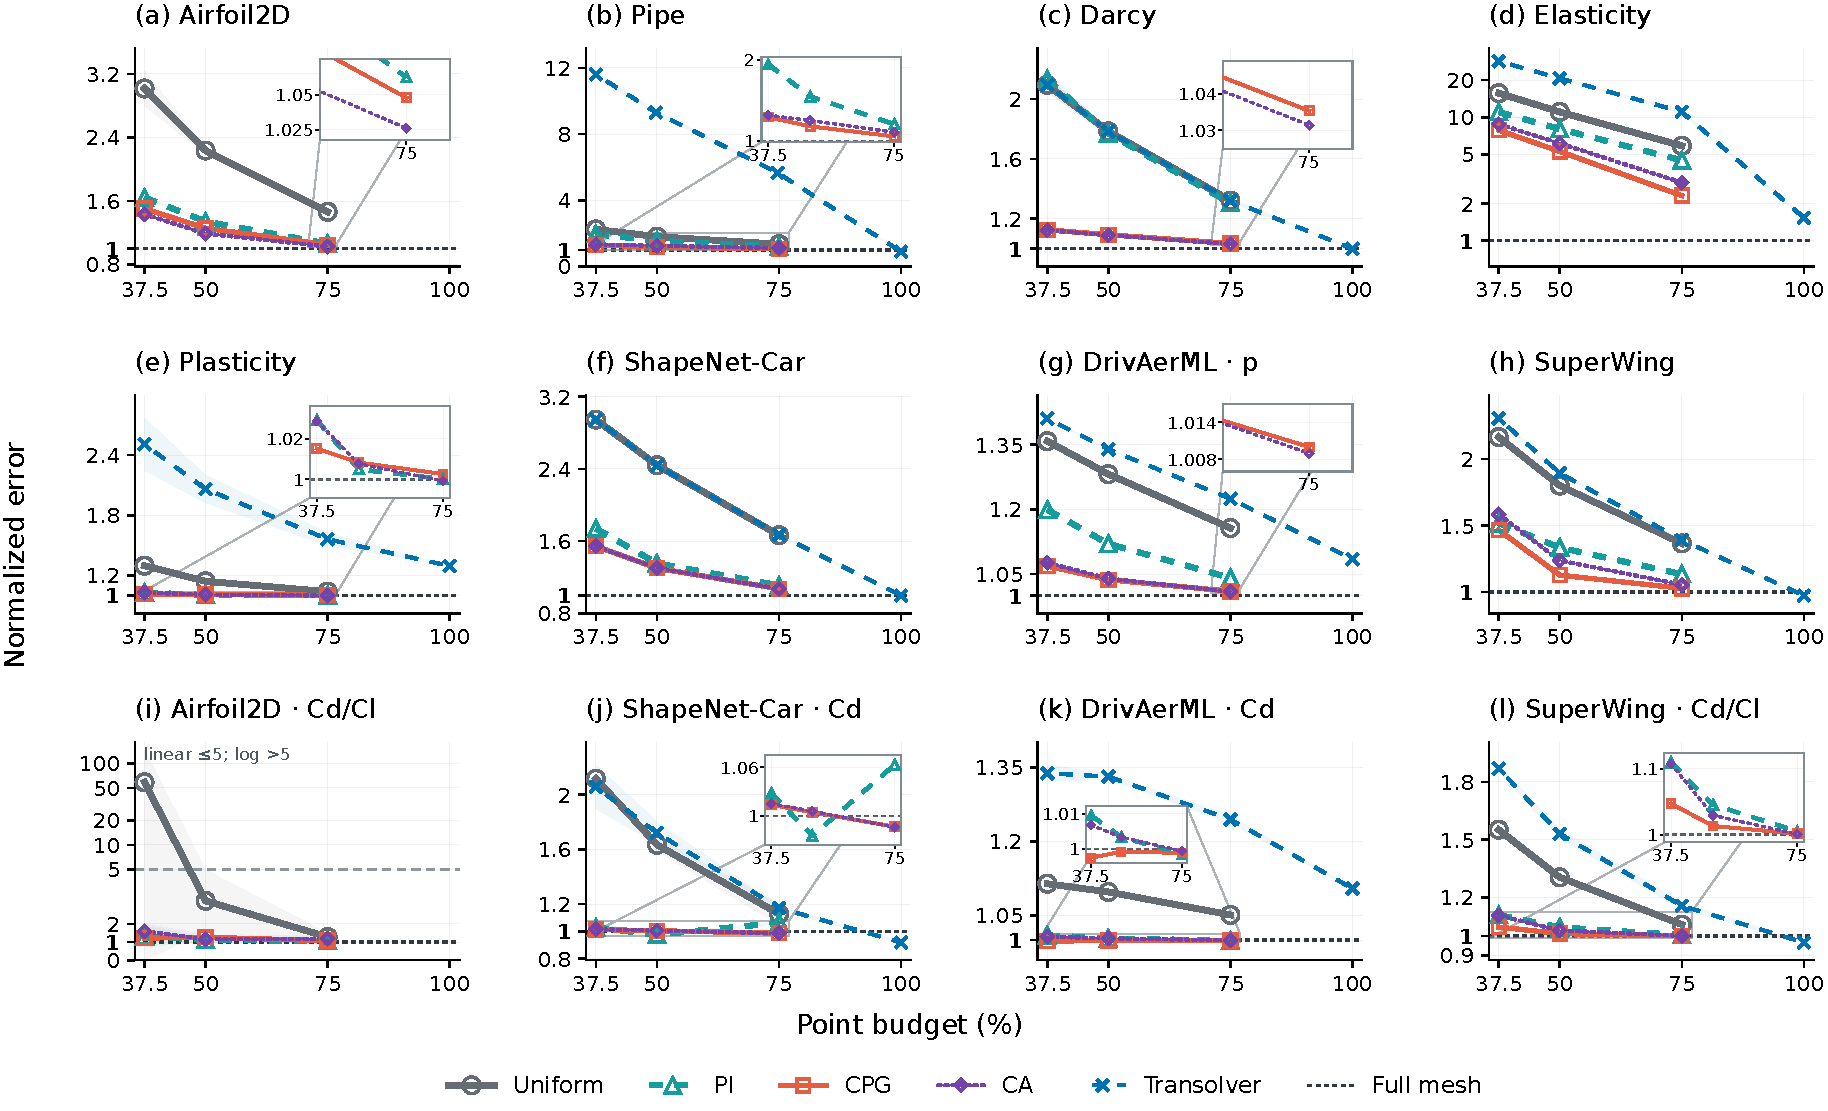
\includegraphics[width=\linewidth]{figures/appendix/budget_error_curves.pdf}
    \caption{\textbf{Error relative to the full mesh across point budgets.}
    Panels (a)--(h) show field metrics and (i)--(l) show aerodynamic quantities.
    Error definitions follow Section~\ref{sec:experiment_implementation}.
    Curves show means over three sampling seeds, with shaded bands indicating
    one sample standard deviation.
    The Airfoil $C_D/C_L$ metric is an absolute coefficient-ratio error before
    normalization, and panel (i) uses a logarithmic vertical axis. The dotted
    line at one marks full-mesh inference accuracy in every panel.}
    \label{fig:appendix_budget_curves}
\end{figure}

\clearpage
\subsection{Additional Field Visualization}
\label{app:field_visualizations}

The following pages connect the aggregate error profiles to spatial sampling
and reconstruction. Each page shows one held-out geometry at a $37.5\%$ point
budget with sampling seed zero. These examples were selected for visible
differences between sampling policies. Their annotations report errors for
the displayed case. The preceding curves summarize the test populations.

The first two rows show sampling locations and the policy's refinement
feature. Features are rescaled from each policy's minimum to its 99th
percentile for display, with larger values clipped at the upper end of the
colour scale. Uniform has no refinement feature. Each physical quantity then
has a ground-truth view and matched prediction and error rows. Field and
error ranges are shared across methods within that quantity. Colour-bar
arrows indicate values outside the displayed range. Component errors are
signed prediction-minus-ground-truth residuals. Magnitude rows show
nonnegative vector error norms, and Plasticity uses the temporal aggregation
specified below.

\subsubsection{Airfoil}
\label{app:vis_airfoil}

The pressure jump in this example makes errors in its location visible as
a narrow residual band. All three adaptive policies reduce the field error
relative to Uniform. PI gives the lowest error for this particular geometry,
illustrating the task-dependent policy ordering seen in the budget curves.

\begin{figure}[!ht]
    \centering
    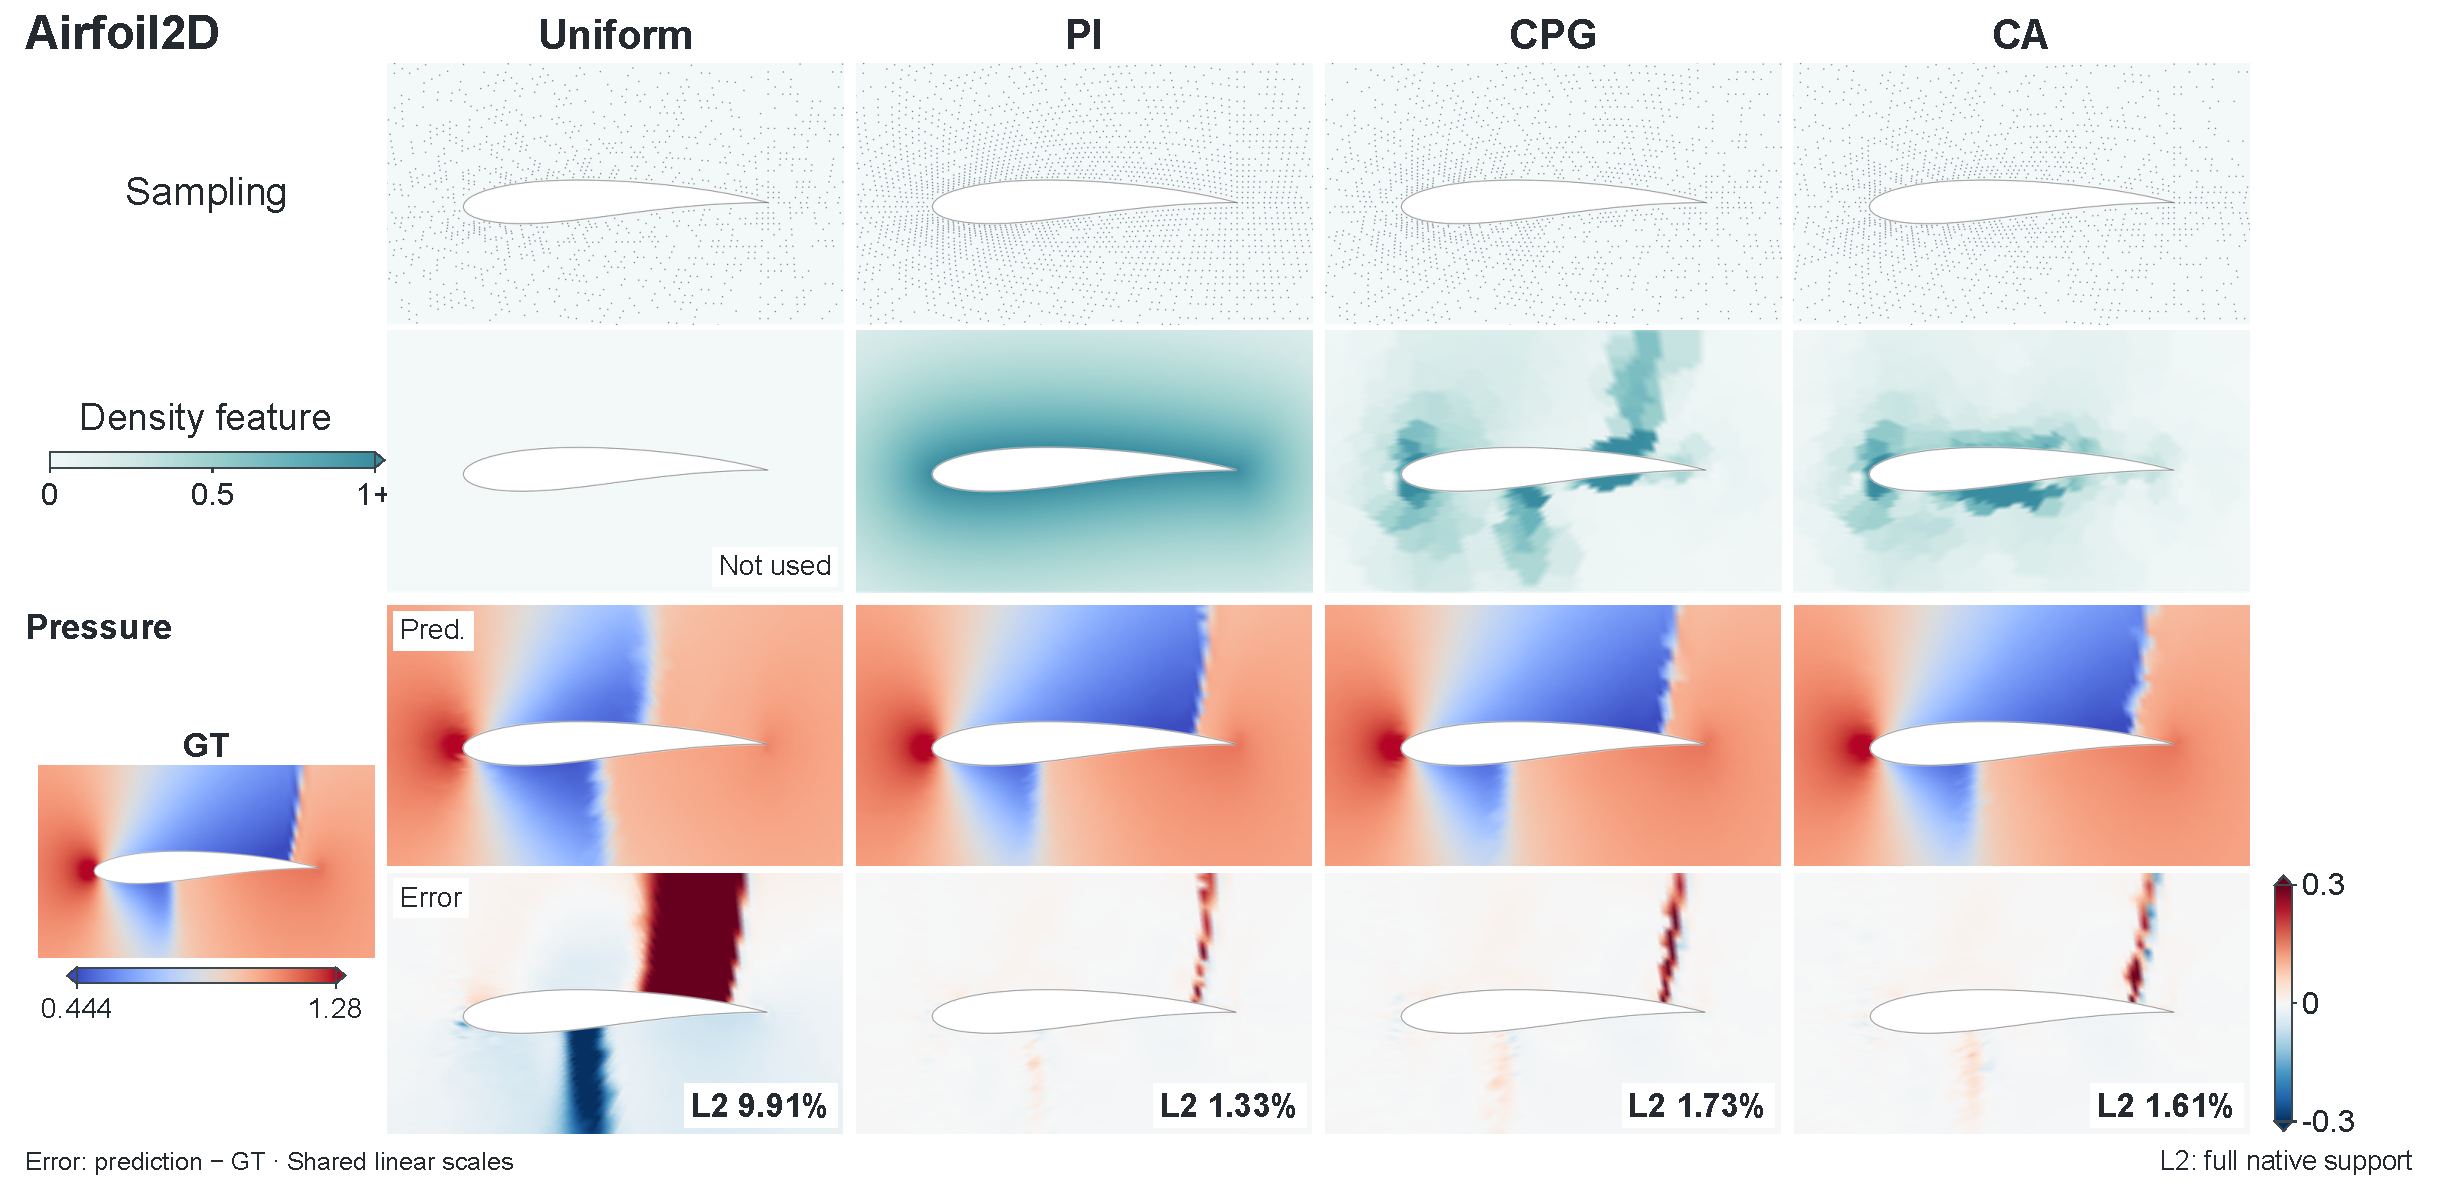
\includegraphics[width=\linewidth,height=.69\textheight,keepaspectratio]{figures/appendix/airfoil2d_fields.pdf}
    \caption{\textbf{Airfoil.} Sampling and pressure prediction.}
    \label{fig:appendix_airfoil}
\end{figure}

\clearpage
\subsubsection{Pipe}
\label{app:vis_pipe}

The predicted horizontal-velocity fields have similar overall structure,
while the shared residual scale exposes differences along the curved pipe.
CPG and CA reduce the error to $0.24\%$ and $0.30\%$, respectively,
compared with $1.31\%$ under Uniform sampling.

\begin{figure}[!ht]
    \centering
    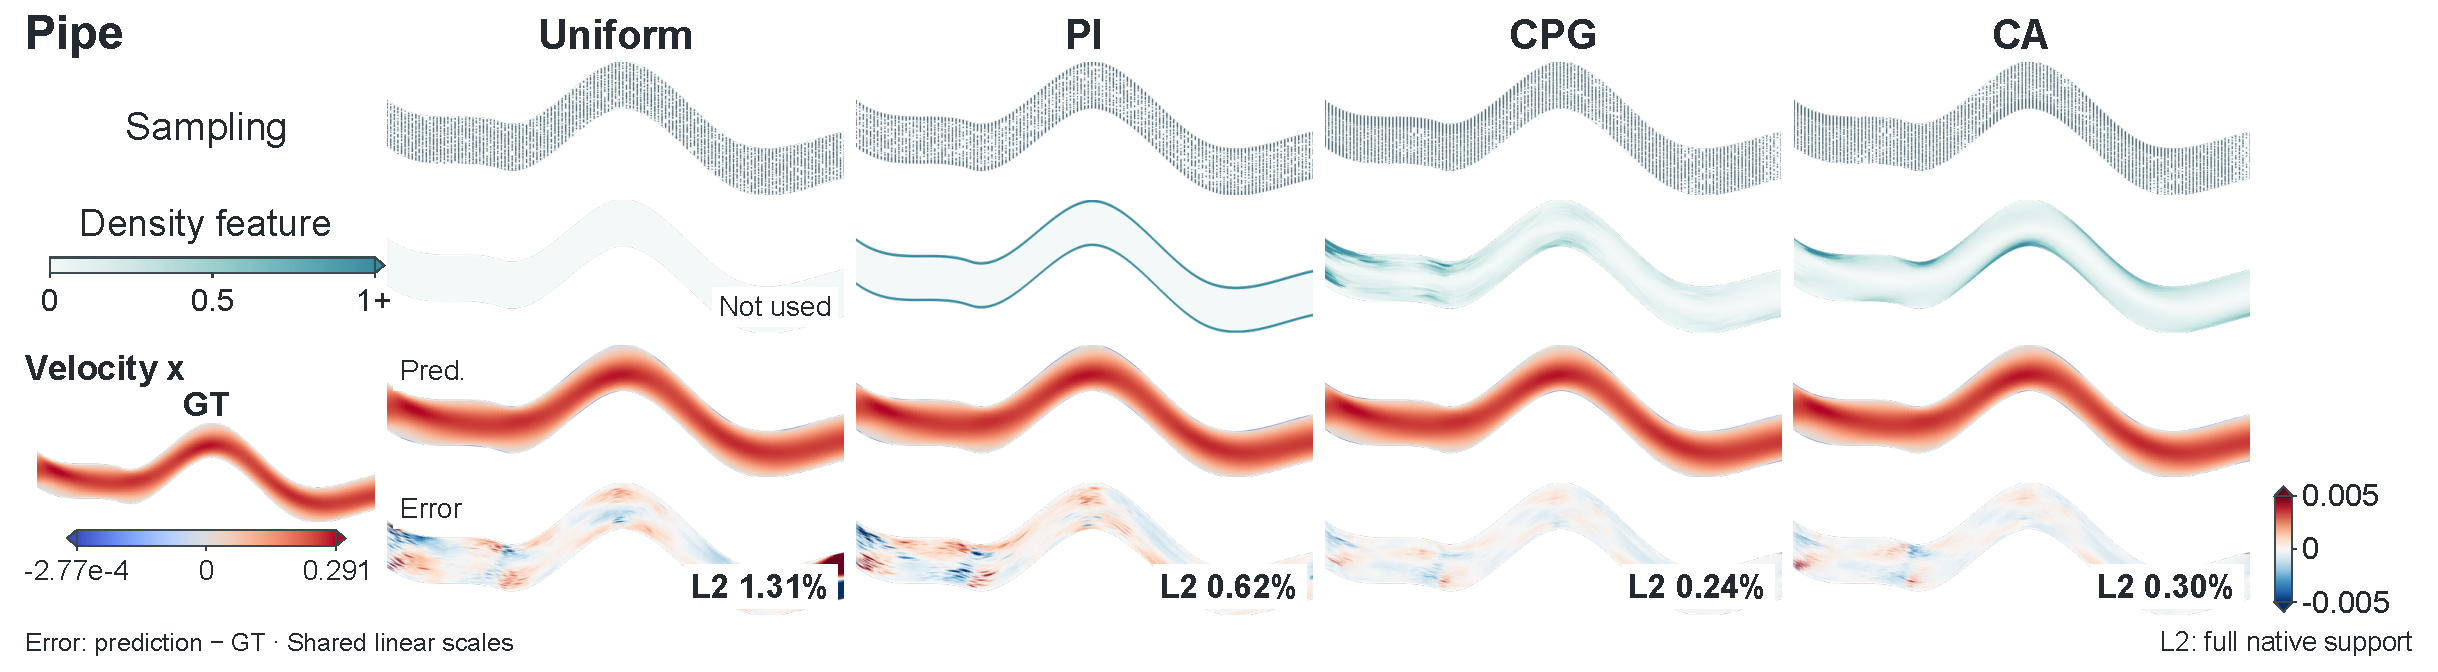
\includegraphics[width=\linewidth,height=.69\textheight,keepaspectratio]{figures/appendix/pipe_fields.pdf}
    \caption{\textbf{Pipe.} Sampling and horizontal velocity prediction.}
    \label{fig:appendix_pipe}
\end{figure}

\clearpage
\subsubsection{Darcy}
\label{app:vis_darcy}

The refinement policies assign different importance to regions of the
heterogeneous medium. The CPG and CA allocations produce similar solution
fields and smaller residuals than Uniform in this example, consistent with
their aggregate advantage on Darcy in Figure~\ref{fig:appendix_budget_curves}.

\begin{figure}[!ht]
    \centering
    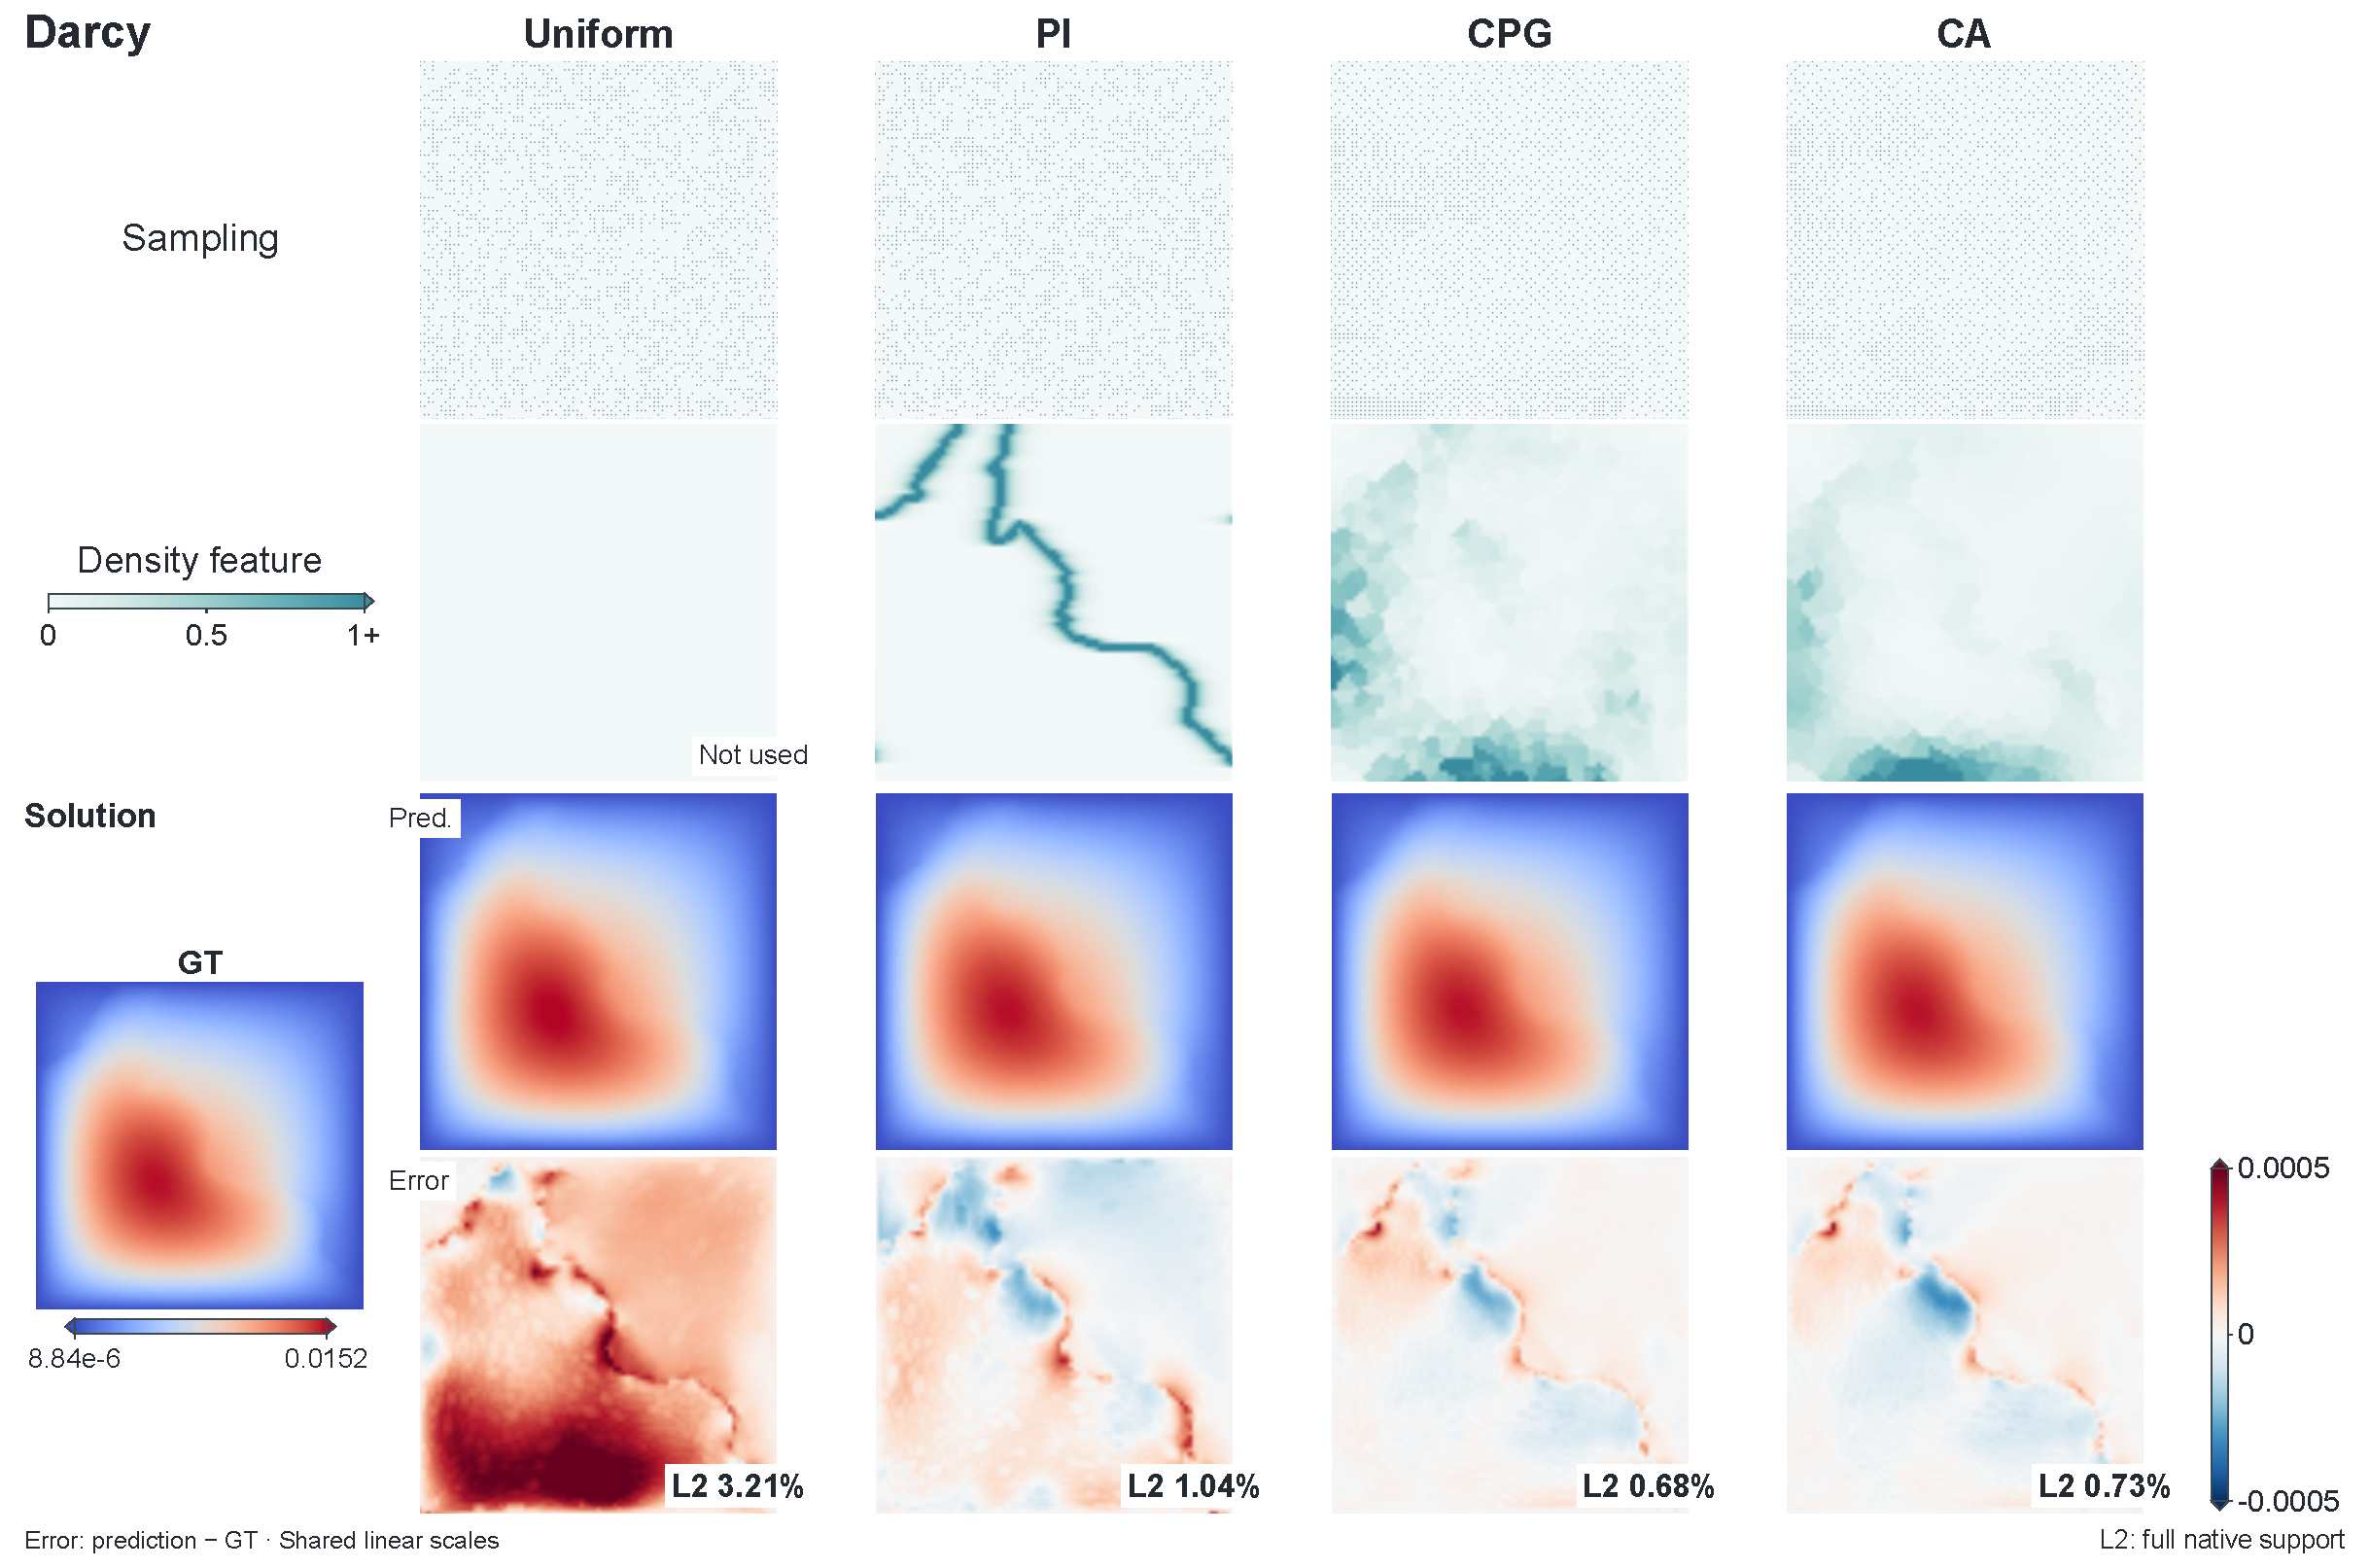
\includegraphics[width=\linewidth,height=.69\textheight,keepaspectratio]{figures/appendix/darcy_fields.pdf}
    \caption{\textbf{Darcy.} Sampling and pressure prediction.}
    \label{fig:appendix_darcy}
\end{figure}

\clearpage
\subsubsection{Elasticity}
\label{app:vis_elasticity}

The irregular hole creates localized stress structure. The residual views
show the reduction in reconstruction error around this region under adaptive
sampling. CPG and CA attain similar errors, with PI also improving
substantially upon the uniform allocation.

\begin{figure}[!ht]
    \centering
    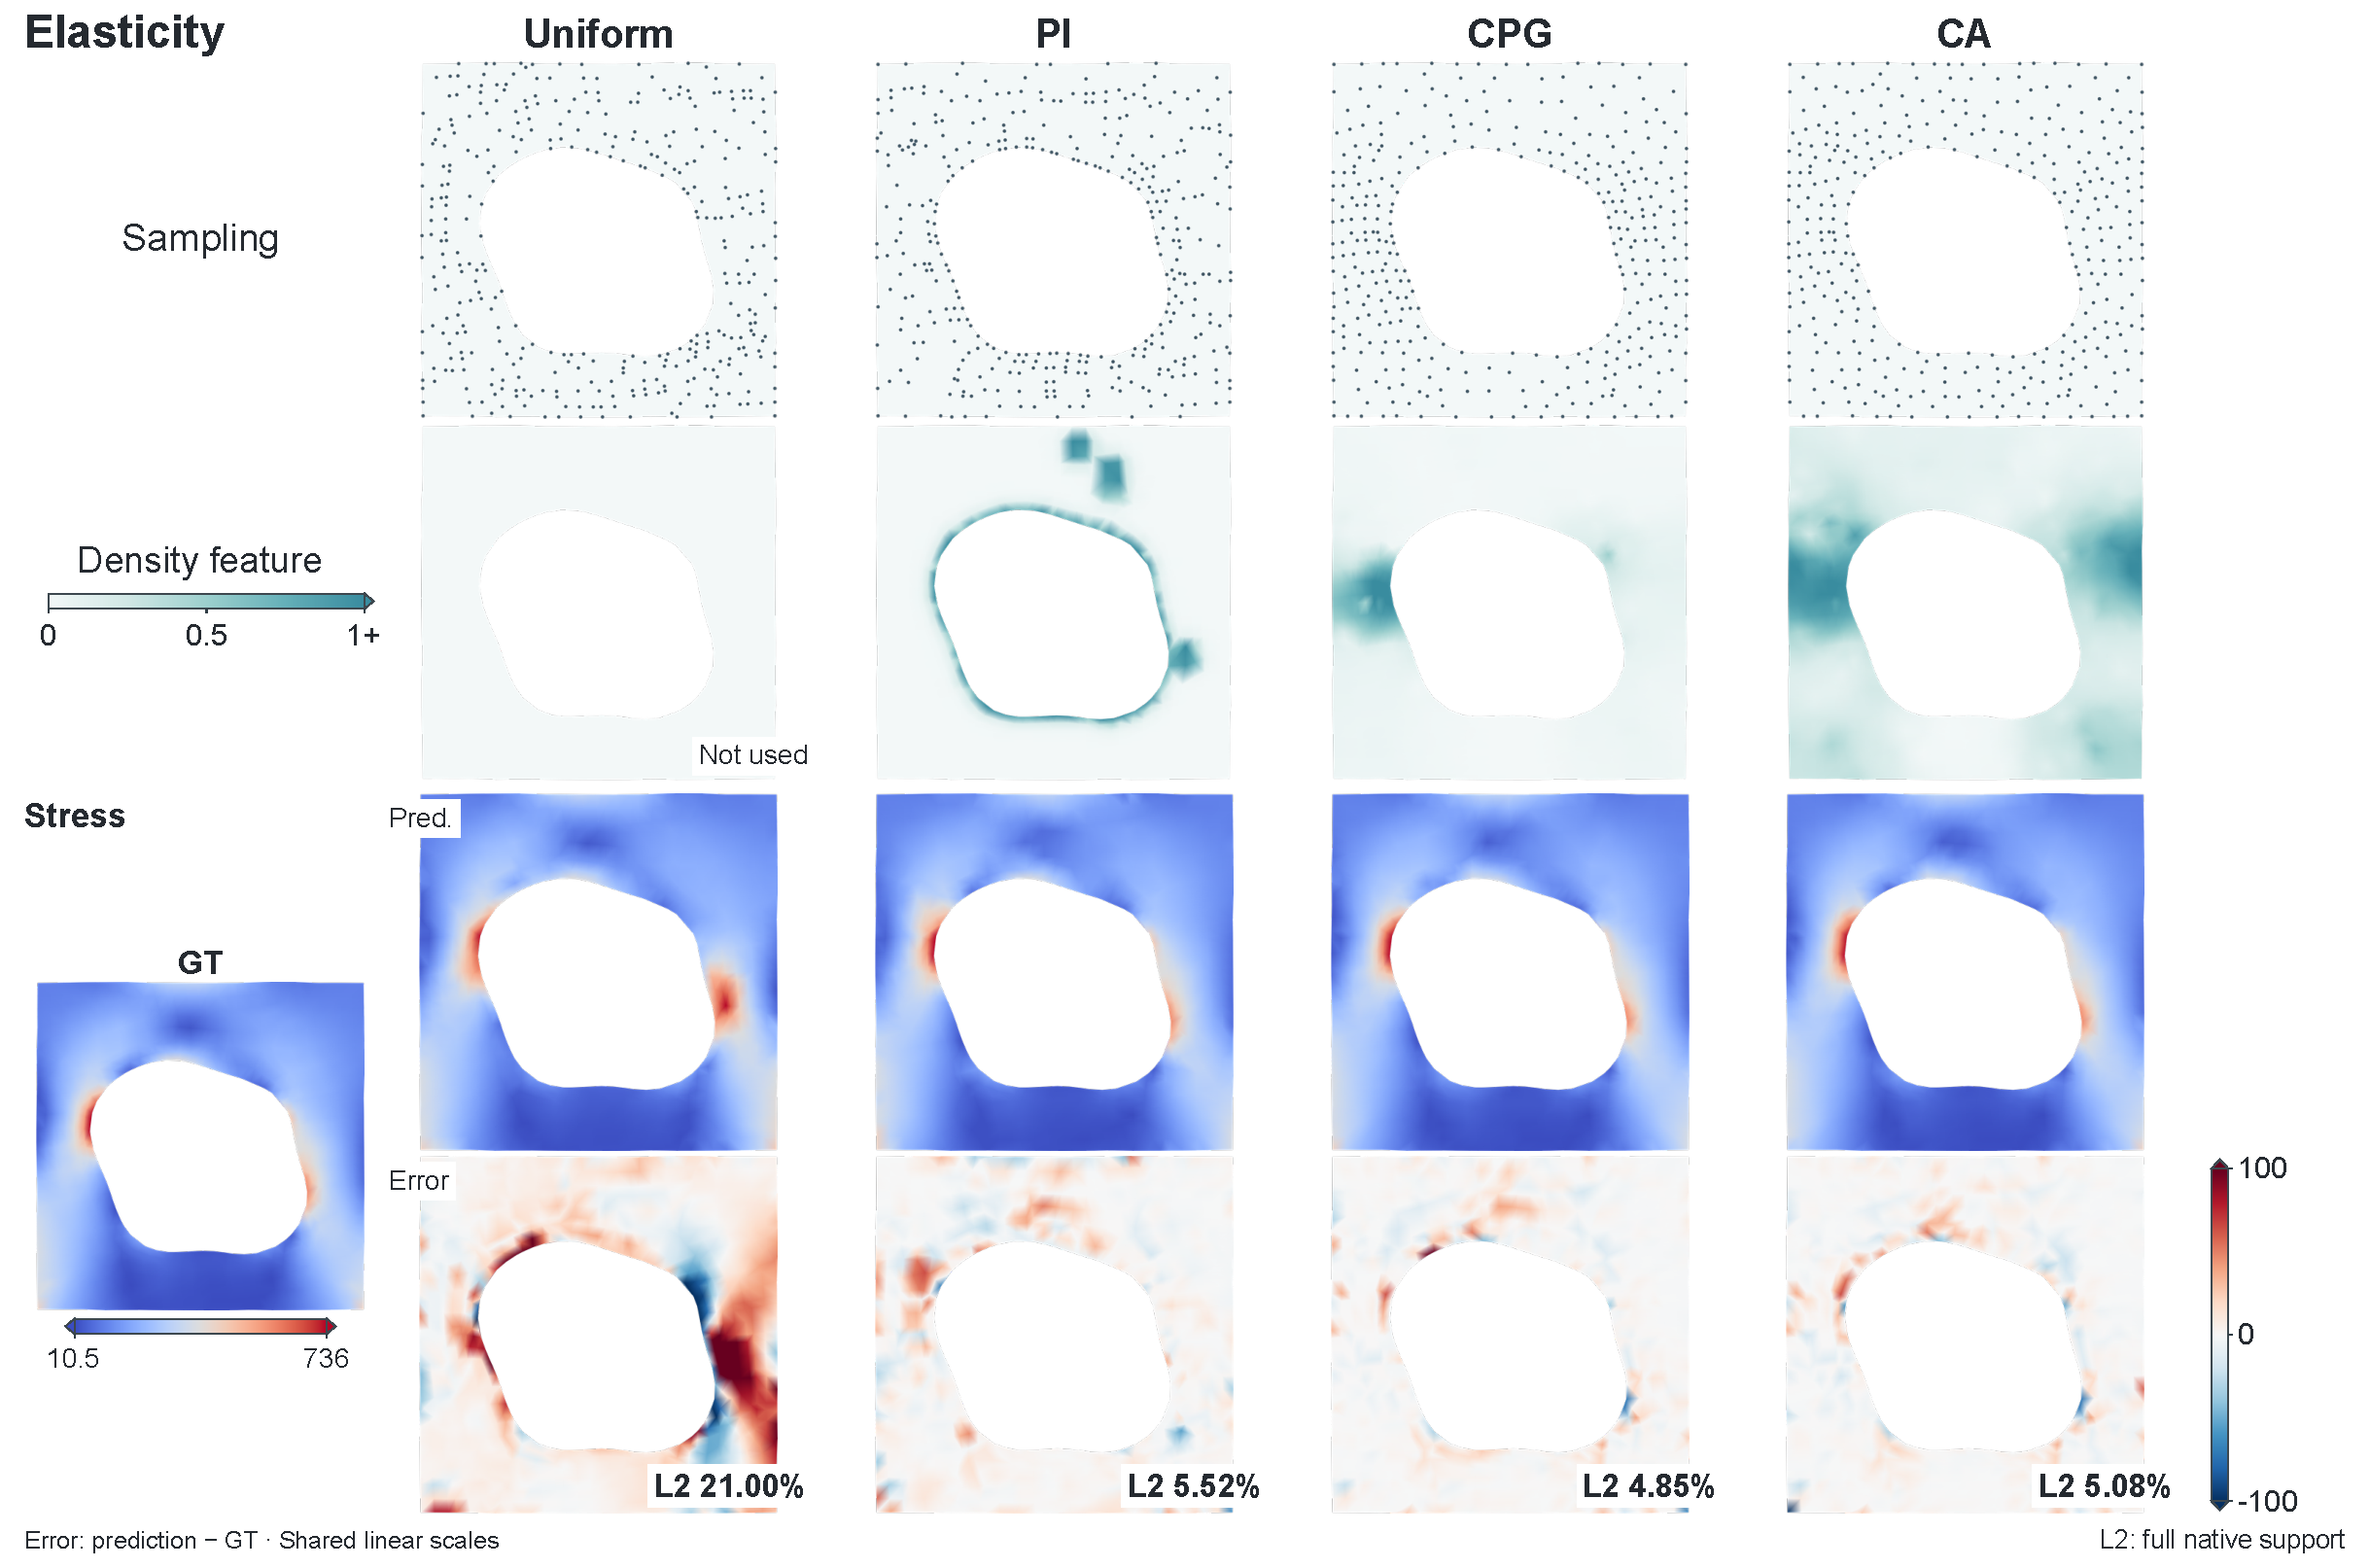
\includegraphics[width=\linewidth,height=.69\textheight,keepaspectratio]{figures/appendix/elasticity_fields.pdf}
    \caption{\textbf{Elasticity.} Sampling and stress prediction.}
    \label{fig:appendix_elasticity}
\end{figure}

\clearpage
\subsubsection{Plasticity}
\label{app:vis_plasticity}

Plasticity predicts a sequence of 20 displacement fields. We summarize all
recorded steps with equal weights, $w_t=1/20$, because the time grid is
uniform. The field rows show time-averaged components and displacement
magnitude. Component-error rows average the absolute residual at each step.
The magnitude-error row averages the vector residual norm. The annotated
$L_2$ errors use the weighted space--time fields over all 20 steps.

\begin{figure}[!ht]
    \centering
    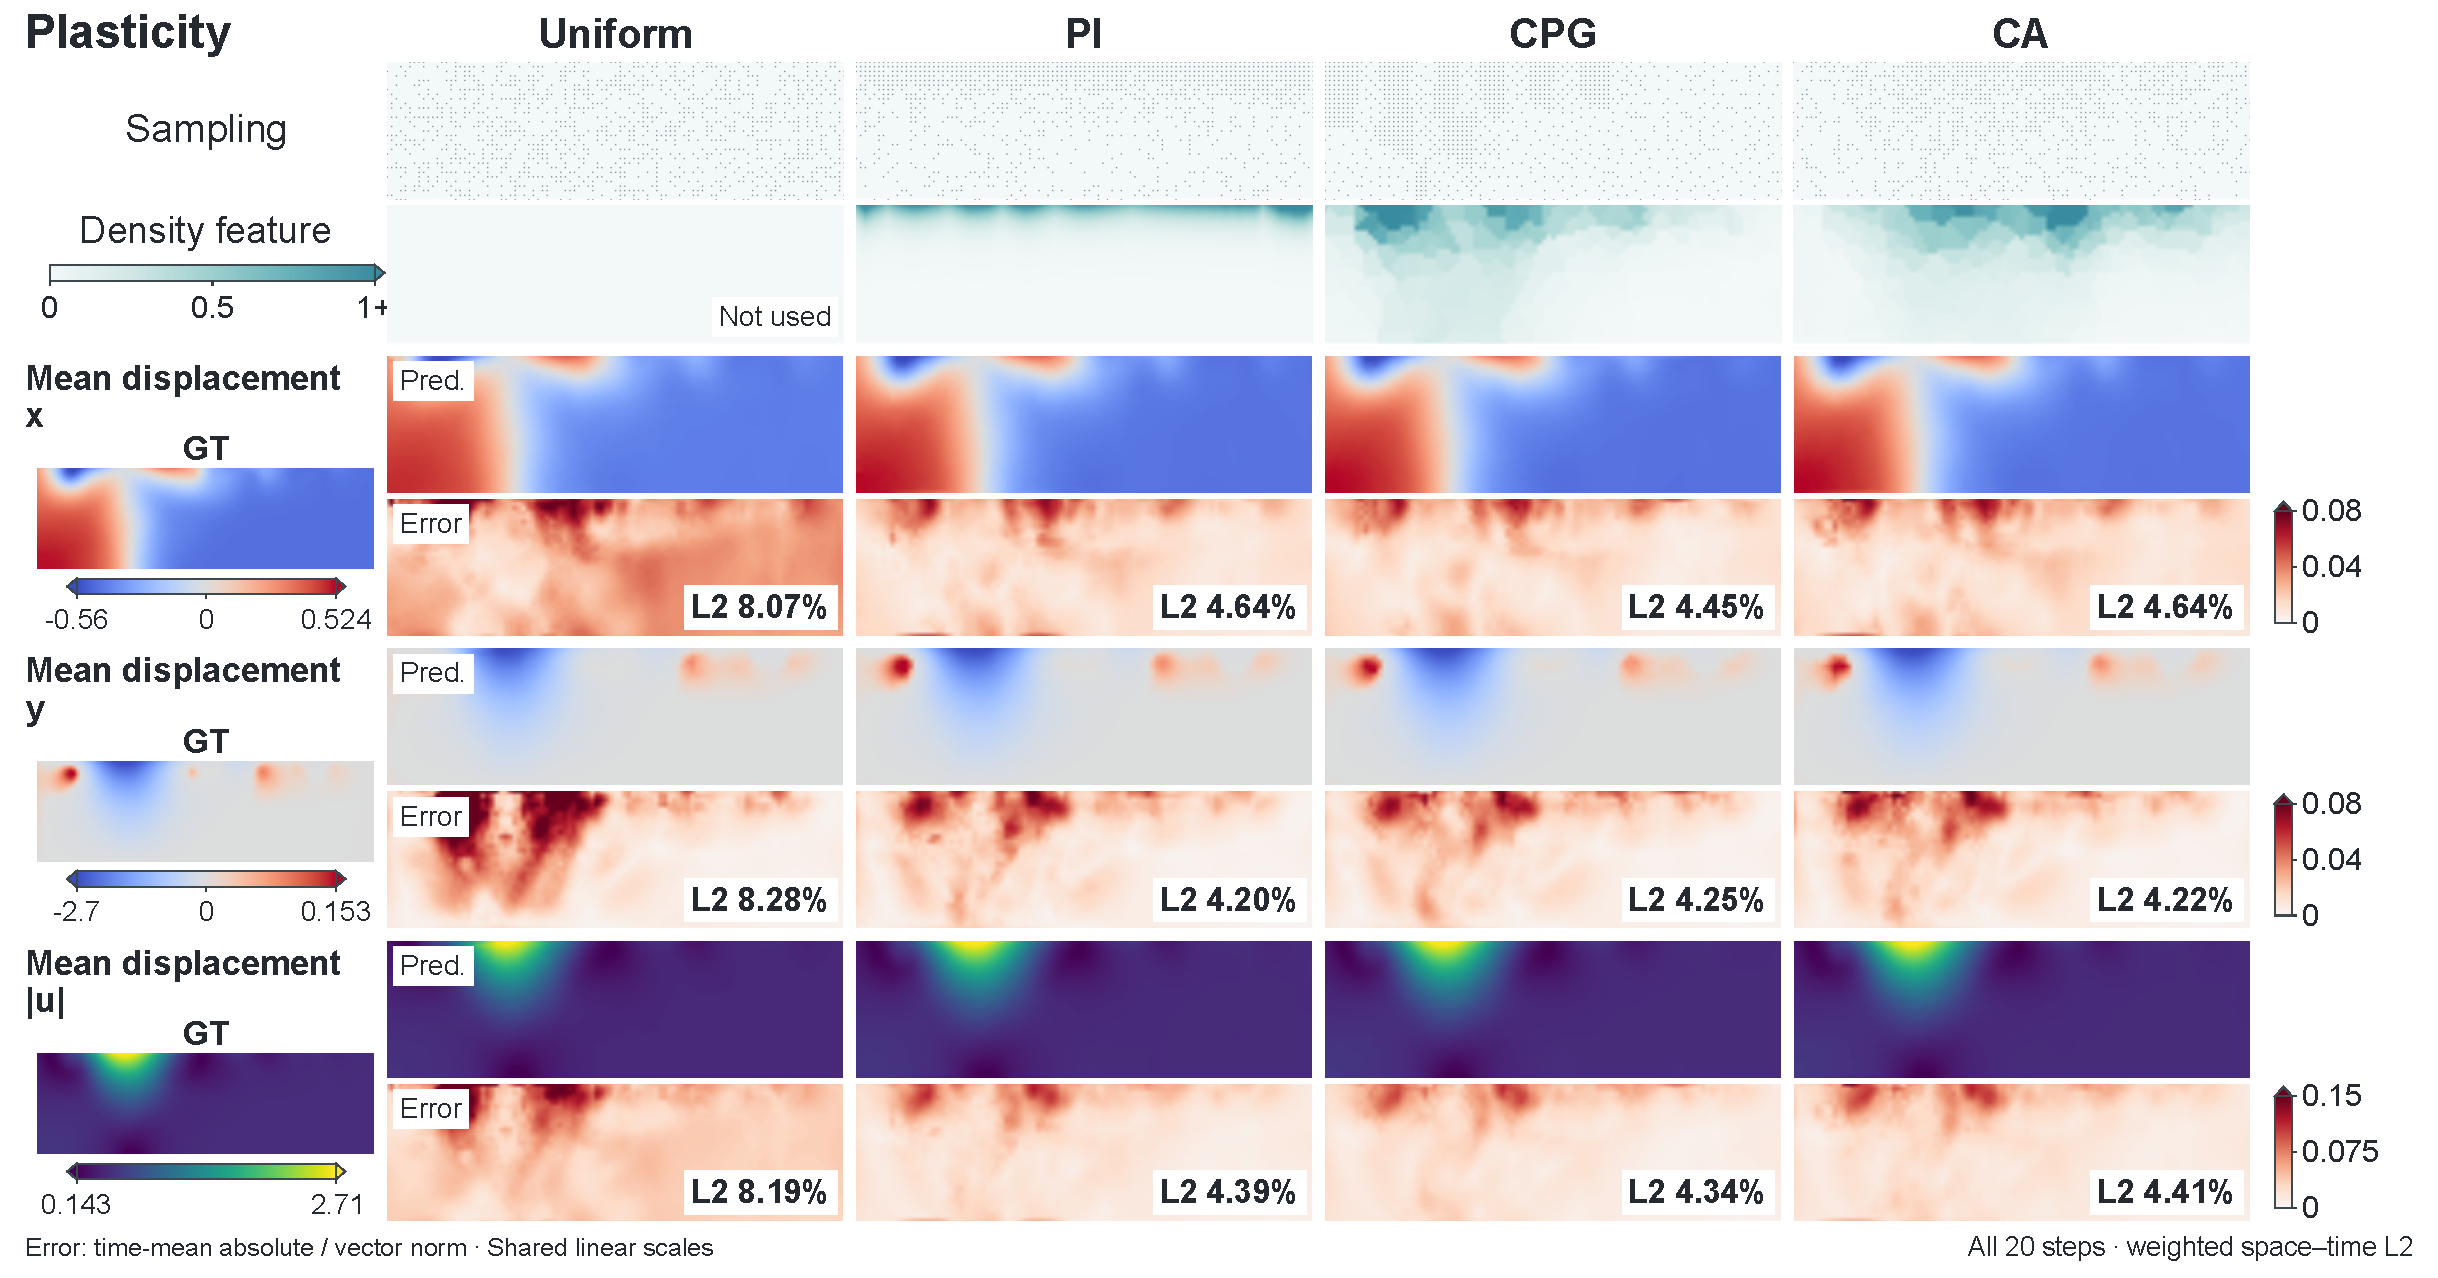
\includegraphics[width=\linewidth,height=.69\textheight,keepaspectratio]{figures/appendix/plasticity2d_fields.pdf}
    \caption{\textbf{Plasticity.} Sampling and displacement prediction.}
    \label{fig:appendix_plasticity}
\end{figure}

\clearpage
\subsubsection{ShapeNet-Car}
\label{app:vis_shapenet}

The automotive examples contain both surface and volumetric outputs.
For ShapeNet-Car, pressure is shown on the surface, and a fixed geometric
slice exposes the three velocity components and speed in the surrounding
volume. Error annotations use each field's full native support. This view
connects changes in point allocation to both pressure and velocity accuracy.

\begin{figure}[!ht]
    \centering
    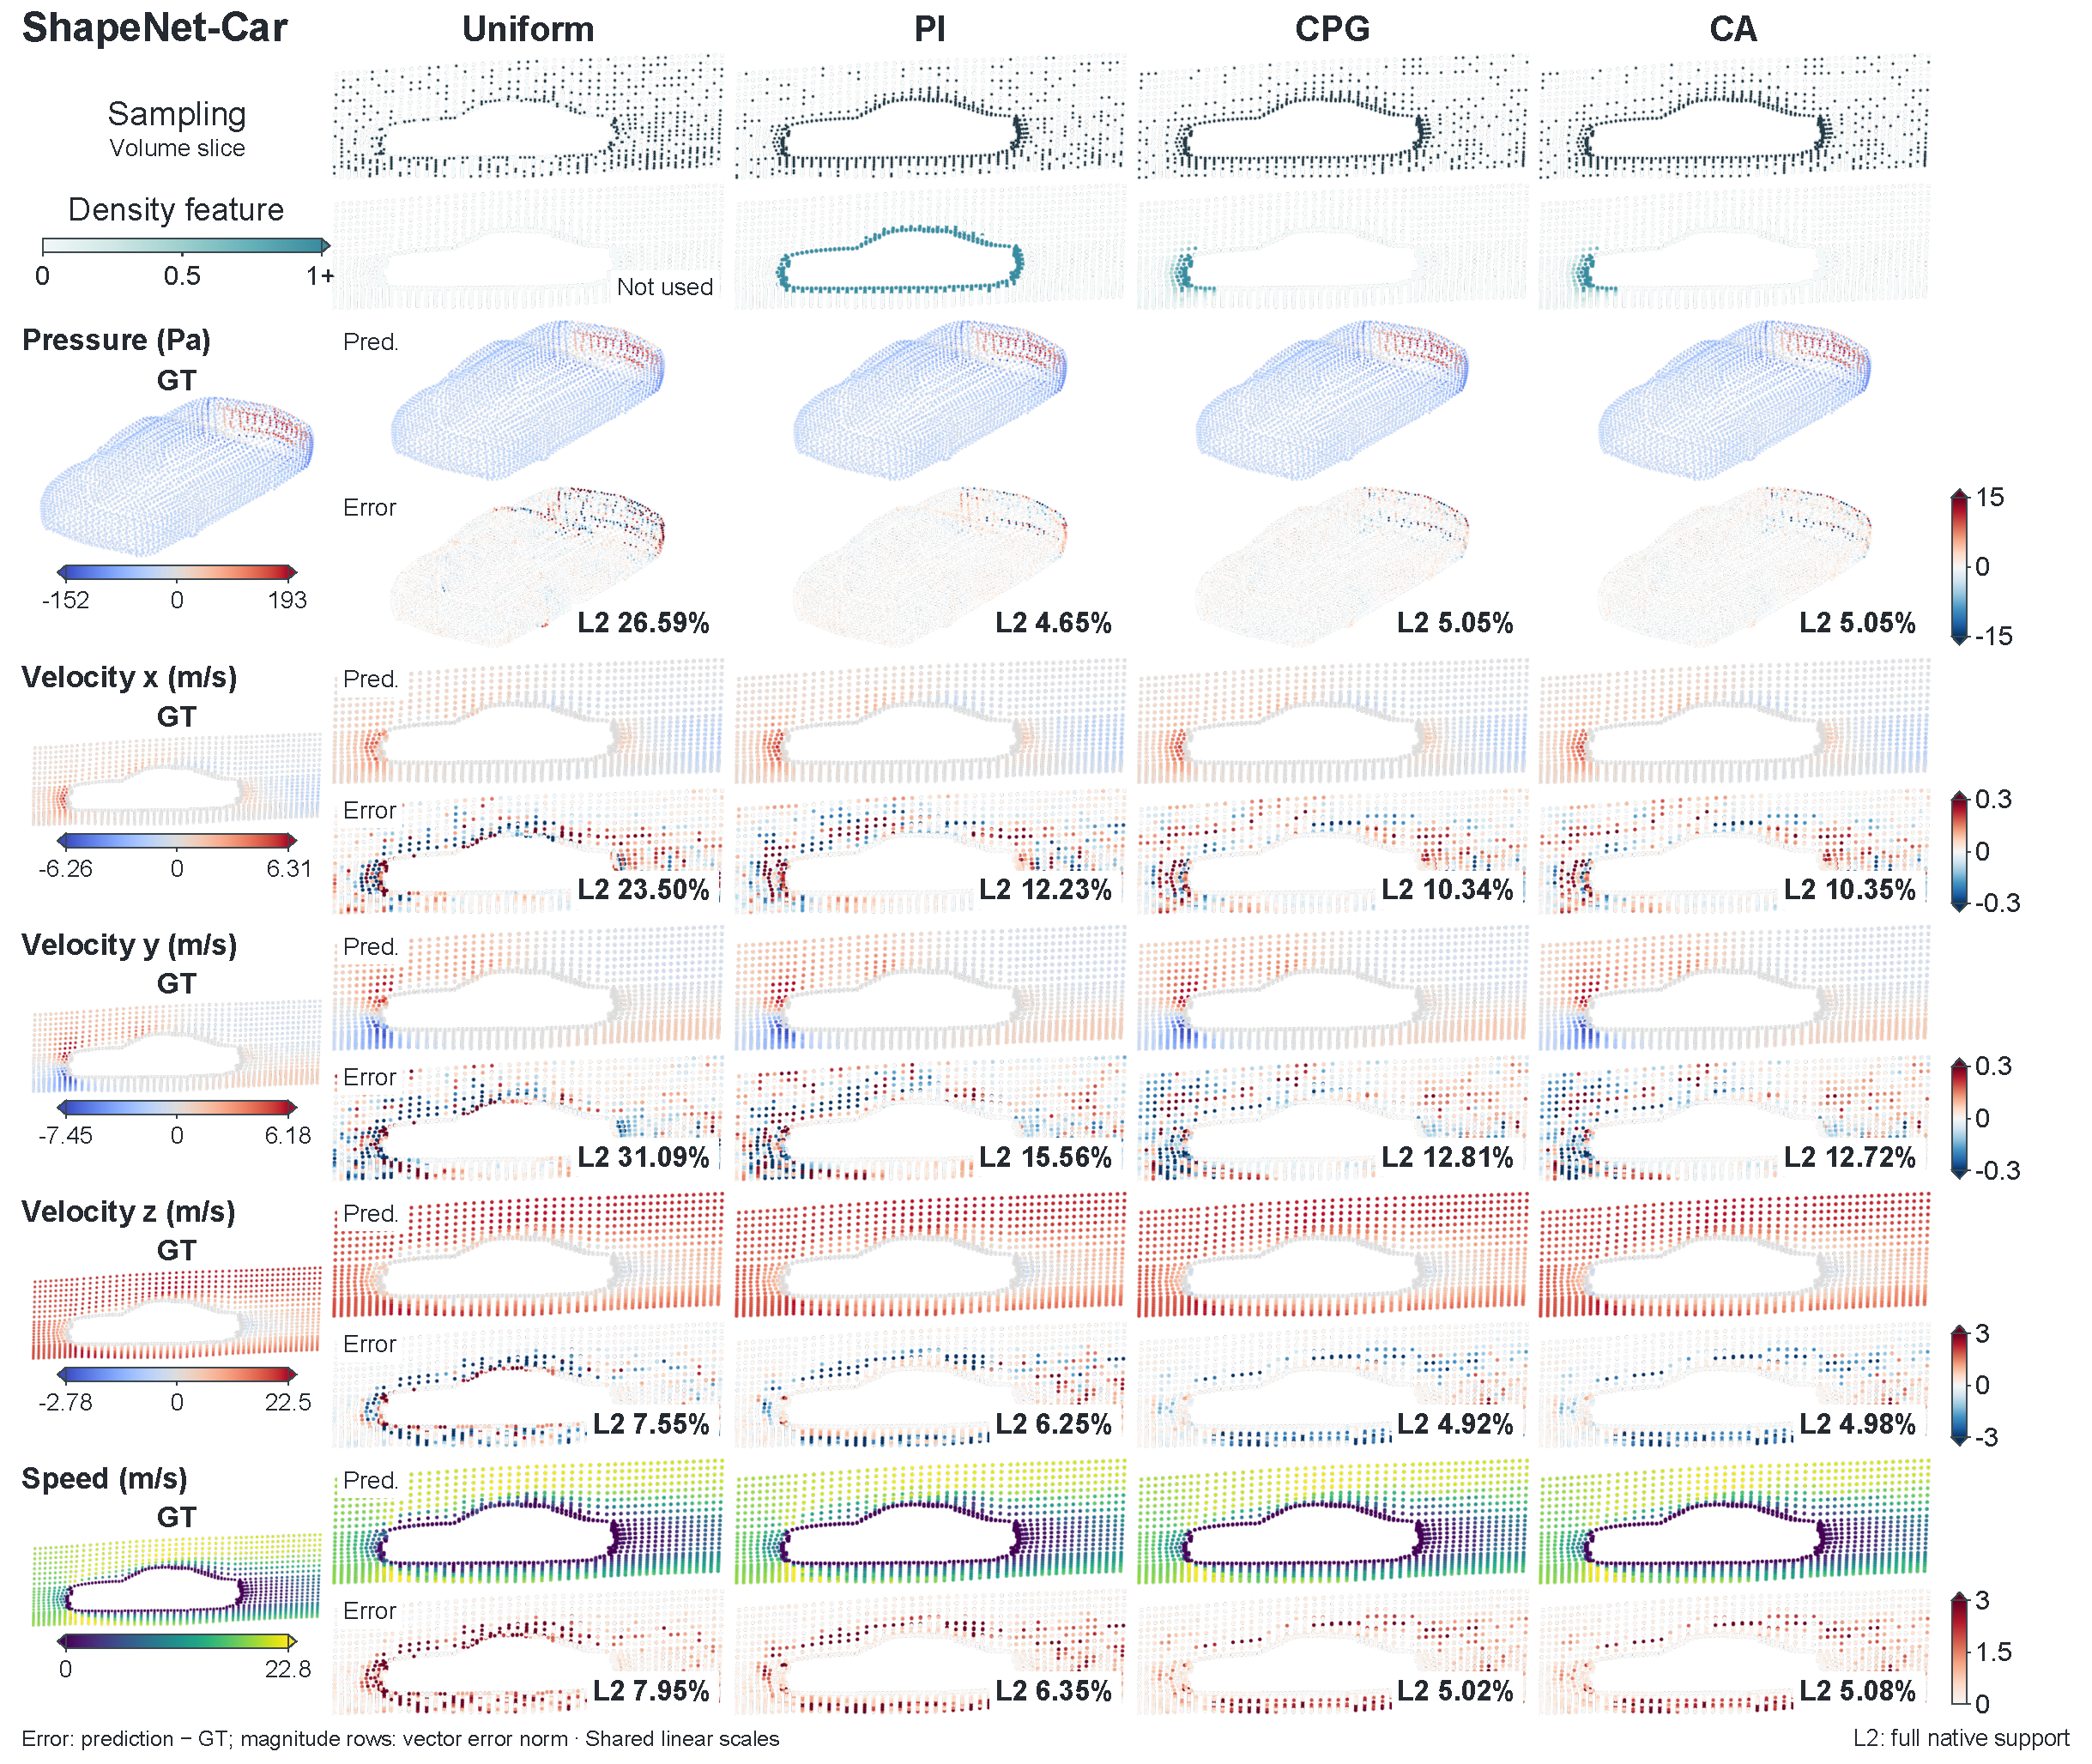
\includegraphics[width=\linewidth,height=.69\textheight,keepaspectratio]{figures/appendix/shapenet_car_fields.pdf}
    \caption{\textbf{ShapeNet-Car.} Sampling and prediction of surface pressure
    and volumetric velocity.}
    \label{fig:appendix_shapenet}
\end{figure}

\clearpage
\subsubsection{DrivAerML}
\label{app:vis_drivaer}

DrivAerML provides pressure and wall-shear-stress predictions on the same
vehicle surface. We reuse each pressure sampler's point indices for the
frozen wall-shear-stress operator. The figure therefore shows how these
allocations affect pressure, all three shear components, and their vector
magnitude on a shared geometry.

\begin{figure}[!ht]
    \centering
    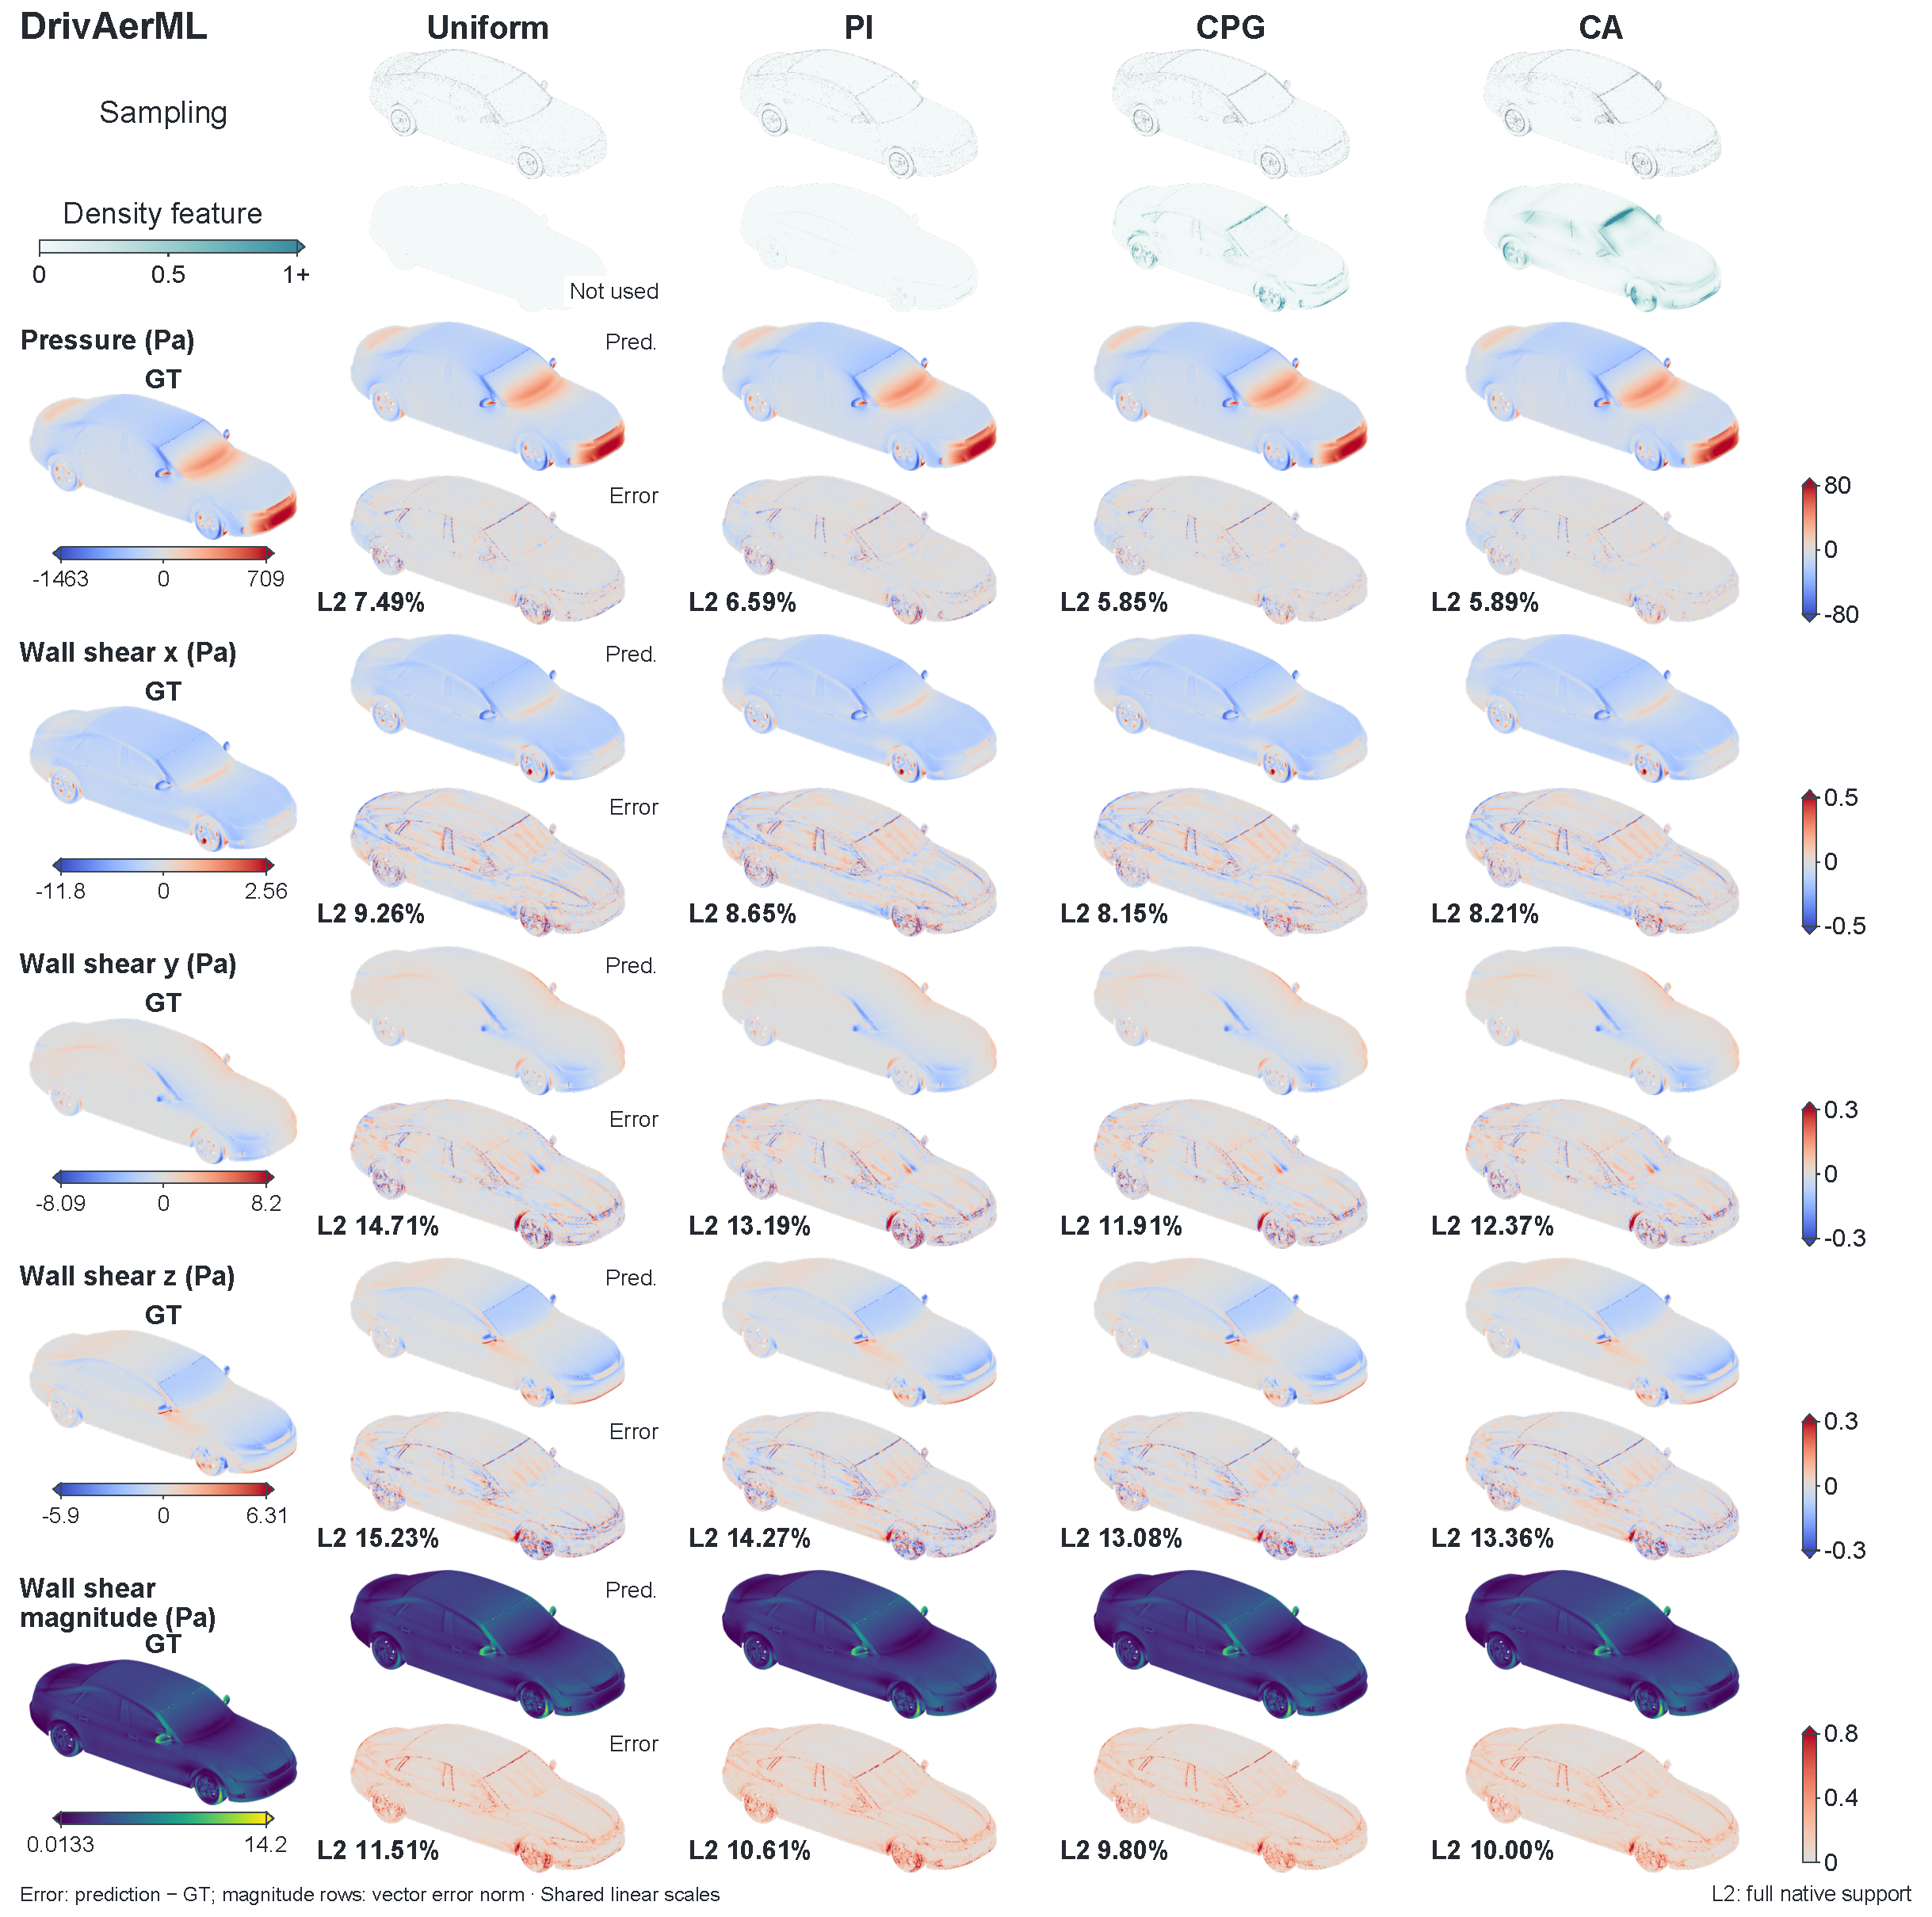
\includegraphics[width=\linewidth,height=.69\textheight,keepaspectratio]{figures/appendix/driverml_fields.pdf}
    \caption{\textbf{DrivAerML.} Sampling and prediction of surface pressure
    and wall shear stress.}
    \label{fig:appendix_drivaer}
\end{figure}

\clearpage
\subsubsection{SuperWing}
\label{app:vis_superwing}

The SuperWing page retains pressure and both friction components, together
with friction magnitude. The stored friction-channel scaling factors are
undone before visualization. Policy ordering varies across these outputs:
CPG gives the smallest pressure error for this wing, while PI gives the
smallest tangent-friction error. The individual rows expose this variation
beyond the joint field metric.

\begin{figure}[!ht]
    \centering
    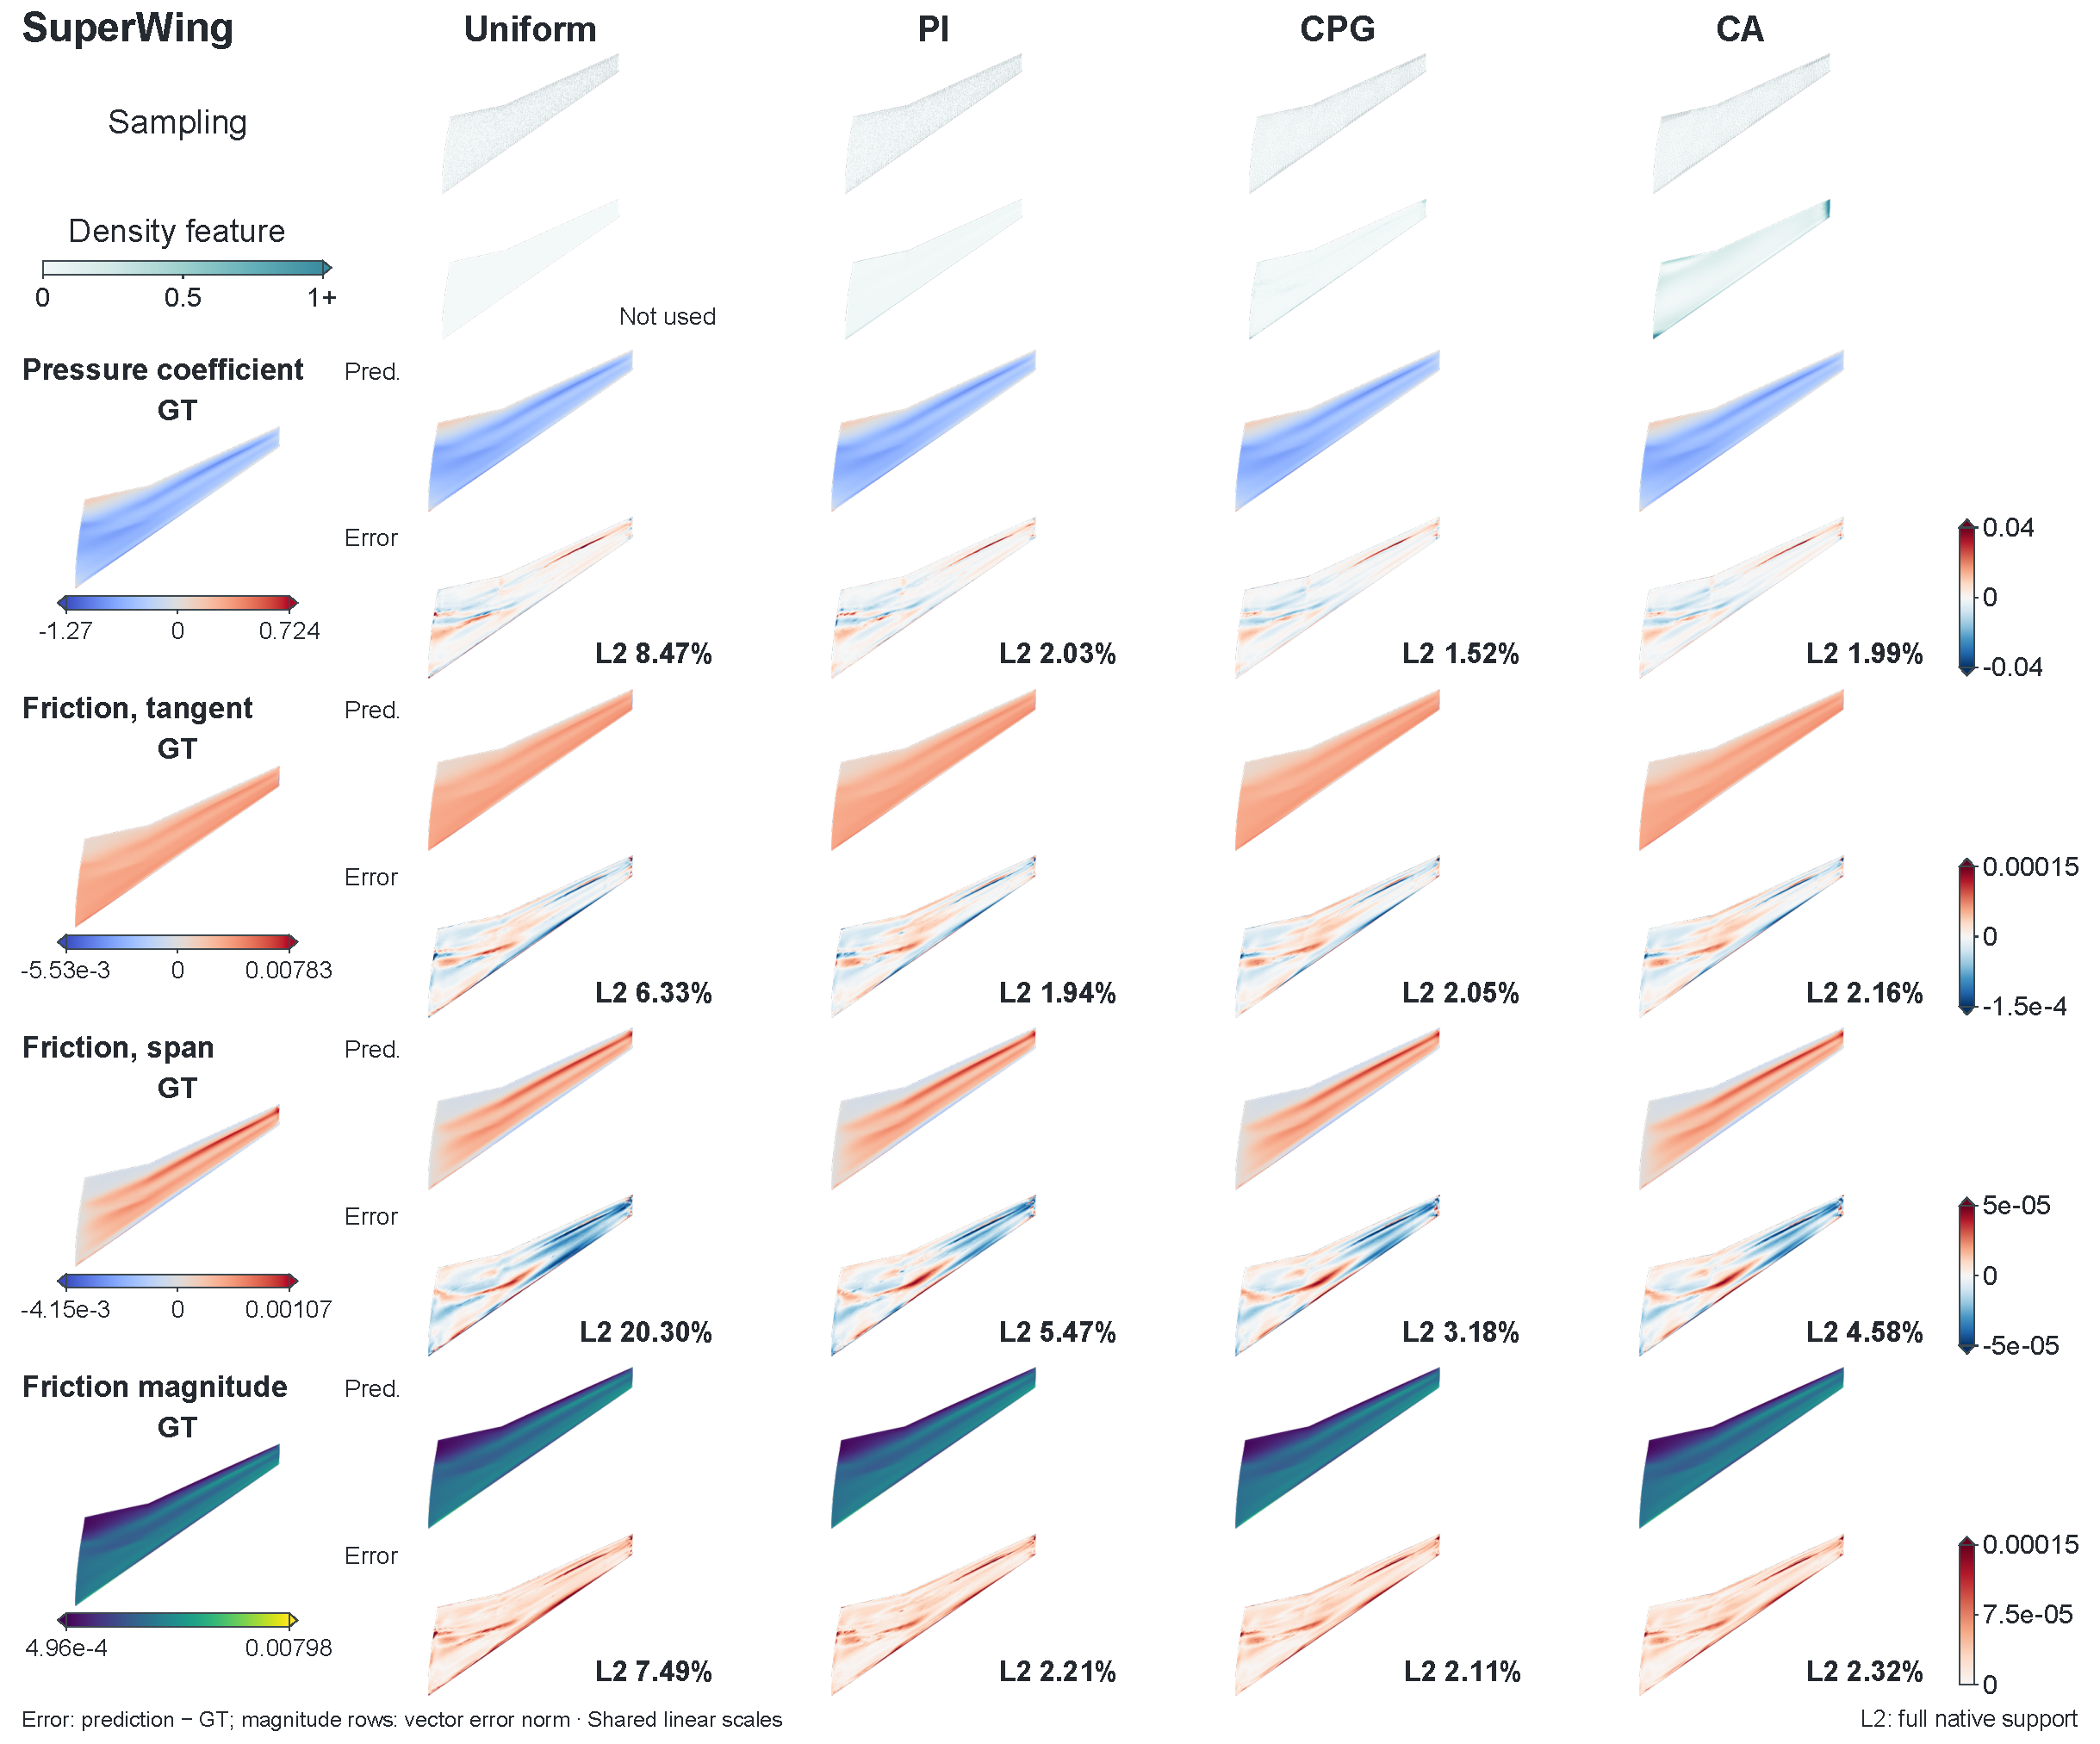
\includegraphics[width=\linewidth,height=.69\textheight,keepaspectratio]{figures/appendix/superwing_fields.pdf}
    \caption{\textbf{SuperWing.} Sampling and prediction of pressure
    and skin-friction coefficients.}
    \label{fig:appendix_superwing}
\end{figure}
